%% This is file `elsarticle-template-5-harv.tex',
%%
%% Copyright 2009 Elsevier Ltd
%%
%% This file is part of the 'Elsarticle Bundle'.
%% ---------------------------------------------
%%
%% It may be distributed under the conditions of the LaTeX Project Public
%% License, either version 1.2 of this license or (at your option) any
%% later version.  The latest version of this license is in
%%    http://www.latex-project.org/lppl.txt
%% and version 1.2 or later is part of all distributions of LaTeX
%% version 1999/12/01 or later.
%%
%% The list of all files belonging to the 'Elsarticle Bundle' is
%% given in the file `manifest.txt'.
%%
%% Template article for Elsevier's document class `elsarticle'
%% with harvard style bibliographic references
%%
%% $Id: elsarticle-template-5-harv.tex 159 2009-10-08 06:08:33Z rishi $
%% $URL: http://lenova.river-valley.com/svn/elsbst/trunk/elsarticle-template-5-harv.tex $
%%
\documentclass[preprint,authoryear,12pt]{elsarticle}
%% Use the option review to obtain double line spacing
%% \documentclass[authoryear,preprint,review,12pt]{elsarticle}

%% Use the options 1p,twocolumn; 3p; 3p,twocolumn; 5p; or 5p,twocolumn
%% for a journal layout:
%% \documentclass[final,authoryear,1p,times]{elsarticle}
%% \documentclass[final,authoryear,1p,times,twocolumn]{elsarticle}
%% \documentclass[final,authoryear,3p,times]{elsarticle}
%% \documentclass[final,authoryear,3p,times,twocolumn]{elsarticle}
%% \documentclass[final,authoryear,5p,times]{elsarticle}
%% \documentclass[final,authoryear,5p,times,twocolumn]{elsarticle}

%% if you use PostScript figures in your article
%% use the graphics package for simple commands
%% \usepackage{graphics}
%% or use the graphicx package for more complicated commands
%% \usepackage{graphicx}
%% or use the epsfig package if you prefer to use the old commands
%% \usepackage{epsfig}

%% The amssymb package provides various useful mathematical symbols
\usepackage{amssymb}
\usepackage{amsmath}
%% The amsthm package provides extended theorem environments
%% \usepackage{amsthm}
\usepackage{color}
\usepackage{siunitx}
\usepackage{array}
\usepackage{lineno}
\usepackage[utf8]{inputenc}
\newcommand{\rpm}{\raisebox{.2ex}{$\scriptstyle\pm$}}
\inputencoding{utf8}
%% The lineno packages adds line numbers. Start line numbering with
%% \begin{linenumbers}, end it with \end{linenumbers}. Or switch it on
%% for the whole article with \linenumbers after \end{frontmatter}.
%% \usepackage{lineno}

%% natbib.sty is loaded by default. However, natbib options can be
%% provided with \biboptions{...} command. Following options are
%% valid:

%%   round  -  round parentheses are used (default)
%%   square -  square brackets are used   [option]
%%   curly  -  curly braces are used      {option}
%%   angle  -  angle brackets are used    <option>
%%   semicolon  -  multiple citations separated by semi-colon (default)
%%   colon  - same as semicolon, an earlier confusion
%%   comma  -  separated by comma
%%   authoryear - selects author-year citations (default)
%%   numbers-  selects numerical citations
%%   super  -  numerical citations as superscripts
%%   sort   -  sorts multiple citations according to order in ref. list
%%   sort&compress   -  like sort, but also compresses numerical citations
%%   compress - compresses without sorting
%%   longnamesfirst  -  makes first citation full author list
%%
%% \biboptions{longnamesfirst,comma}

% \biboptions{}

\journal{Biosystems Engineering}

\begin{document}

\begin{frontmatter}

%% Title, authors and addresses

%% use the tnoteref command within \title for footnotes;
%% use the tnotetext command for the associated footnote;
%% use the fnref command within \author or \address for footnotes;
%% use the fntext command for the associated footnote;
%% use the corref command within \author for corresponding author footnotes;
%% use the cortext command for the associated footnote;
%% use the ead command for the email address,
%% and the form \ead[url] for the home page:
%%
%% \title{Title\tnoteref{label1}}
%% \tnotetext[label1]{}
%% \author{Name\corref{cor1}\fnref{label2}}
%% \ead{email address}
%% \ead[url]{home page}
%% \fntext[label2]{}
%% \cortext[cor1]{}
%% \address{Address\fnref{label3}}
%% \fntext[label3]{}

% \title{An Autonomous Platform for Use in Kiwifruit Orchards}
\title{A Heavy-Duty Modularised Platform for Autonomous Navigation in Kiwifruit Orchards}

%% use optional labels to link authors explicitly to addresses:
%% \author[label1,label2]{<author name>}
%% \address[label1]{<address>}
%% \address[label2]{<address>}

% \author{Mark H. Jones, Jamie Bell, Matthew Seabright, Joshua Barnett, Alistair Scarfe, Bruce MacDonald, Mike Duke}

%% Group authors per affiliation:
\author[UoW]{Mark H. Jones\corref{mjemail}}
\cortext[mjemail]{MarkHedleyJones@gmail.com}

\author[UoA]{Jamie Bell\corref{jbemail}}
\cortext[jbemail]{jamie977@gmail.com}
\author[UoW]{Matthew Seabright}
\author[RPL]{Alistair Scarfe}
\author[UoW]{Mike Duke}
\author[UoA]{Bruce MacDonald}

\address[UoW]{School of Engineering, University of Waikato, Hamilton, New Zealand}
\address[UoA]{Faculty of Engineering, University of Auckland, Auckland, New Zealand}
\address[RPL]{Robotics Plus Ltd, Newnham Innovation Park, Tauranga, New Zealand}


\begin{abstract}
%% Text of abstract
    Horticutural robots designed for in-field use generally require a means of locomotion through farms or orchards.
    % Robotic systems for horticulture use generally require a means of locomotion through farms or orchards.
    A common approach is to directly integrate a drive system at the expense of increasing overall complexity.
    While general purpose platforms have been reported previously, they are mostly developed for use with open field crops and not for carrying heavy payloads.
    This paper presents a platform capable of carrying a \SI{1000}{\kilo\gram} payload through GNSS-denied environments, autonomously.
    The platform is general in the sense that it itself does not perform tasks.
    It is intended solely to navigate through pergola style orchards while being capable of carrying and supplying power to mounted modules.
    Navigation sensor selection with in-orchard validation tests are presented.




    % \color{red}Mention that the vehicle operates in a GPS-denied environment\color{black}.
    % Systems for performing autonomous horticultural tasks usually require a means of locomotion through their environment.
    % One approach is to directly integrate a drive system at the expense of increasing overall complexity and development risk.
    % We present a generalised mobile platform designed to carry task specific robots through pergola style kiwifruit orchards.
    % The platform is general in the sense that it itself does not perform tasks.
    % It is intended solely to navigate through orchards and be capable of carrying robotic modules.

    % The selection of sensors best suited for autonomous navigation in this environment is discussed and presented with in-orchard test results.
    % Details of the platform's software and hardware architecture are also discussed.
    % The series-hybrid platform presented here has reliably self-navigated through two test orchards unassisted and is capable of carrying a \SI{1000}{\kilo\gram} payload.
\end{abstract}

\begin{keyword}
%% keywords here, in the form: keyword \sep keyword

%% MSC codes here, in the form: \MSC code \sep code
%% or \MSC[2008] code \sep code (2000 is the default)
    Agricultural automation \sep autonomous navigation \sep orchard robotics \sep sensor selection
\end{keyword}

\end{frontmatter}

\linenumbers
% \linenumbers

%% main text
\section{Introduction}
\label{sect:intro}
    Short-term labor requirements within New Zealand's kiwifruit industry peak twice a year corresponding with the pollination and harvesting of kiwifruit.
    The majority of employment during these peaks is filled by seasonal or casual workers \citep{Timmins2009}.
    As kiwifruit is the country's largest horticultural export by value \citep{StatisticsNewZealand2015}, effective automation in this industry will promote economic growth.
    % The New Zealand government aims to double exports from its primary industries between 2012 and 2025 and is actively investing in programmes to achieve this \citep{MinistryPrimaryIndustries2015}.

    Research towards automated kiwifruit harvesting on a purpose built platform has previously been demonstrated \citep{Scarfe2012}.
    That work presented a platform designed to autonomously navigate though pergola style kiwifruit orchards and featured four integrated harvesting arms.
    % The pergola is the most commonly used support structure used to grow kiwifruit in New Zealand.
    Work presented here focuses on developing a platform independently from tasks such as harvesting and pollination.
    This means increasing modularity by separating the task specific systems from the base platform.
    % Harvesting and pollination modules designed for use on the platform have been published elsewhere \citep{williams2017,Seabright2017}.
    Details of harvesting and pollination modules designed for the platform will be published separately.
    These task specific modules have been designed in parallel with the platform as part of a larger project focusing on automation in kiwifruit orchards.

    % Automation in kiwifruit harvesting and pollination demands computer control, state-of-the-art manipulators, and machine-vision based identification systems.
    Automated kiwifruit harvesting and pollination demands computer control, state-of-the-art manipulators, and machine-vision systems.
    Such systems are bulky and have specific geometric requirements dictated by the environment they operate in.
    Both share the need for electrical power, air pressure, and a means of locomotion.
    However, they differ in the way they move when operating.
    The pollinating module moves at a well-known velocity with minimum changes in angle.
    This differs from the harvesting module that advances a set distance between stationary harvest cycles.
    To enable the whole system to work autonomously, the base platform must be able to self-drive in a way appropriate for these modules.

    It has been stated that ``since the robot development already includes a high complexity, the application itself should be of comparably low complexity'' \citep{Ruckelshausen2009}.
    By separating the development of the platform from other task-specific modules, the risk of a single part becoming overly complex is reduced.
    The platform presented here simply needs to navigate through orchards.

    The development of autonomous vehicles in agriculture is not new, but much of the literature relates to manned vehicles converted to drive-by-wire.
    Because the canopy of a pergola style kiwifruit orchard can droop as low as \SI{1.5}{\meter} to the ground under fruit loading, most standard vehicles are unsuitable for use this environment.
    Many autonomous vehicles designed for use in orchards, such as vineyards, rely on satellite navigation for guidance.
    The dense foliage of a kiwifruit canopy and the surrounding shelter-belts make receiving satellite navigation signals unreliable at best.

    This paper presents a modularised platform built specifically for use in pergola style orchards.
    Capability requirements for the platform are to:
    \begin{enumerate}
        \item be weatherproof,
        \item support a total mass of \SI{1000}{\kilo\gram},
        \item be no more than \SI{1.4}{\meter} in height,
        \item supply \SI{10}{\kilo\watt} of electrical power,
        \item power itself for at least eight hours,
        \item turn between rows in orchard headland areas,
        \item include a bin-lifting mechanism for carrying fruit bins, and
        \item provide a module mounting area no more than \SI{400}{\milli\meter} from the ground.
    \end{enumerate}
    \begin{figure}[htb]
        \centering
        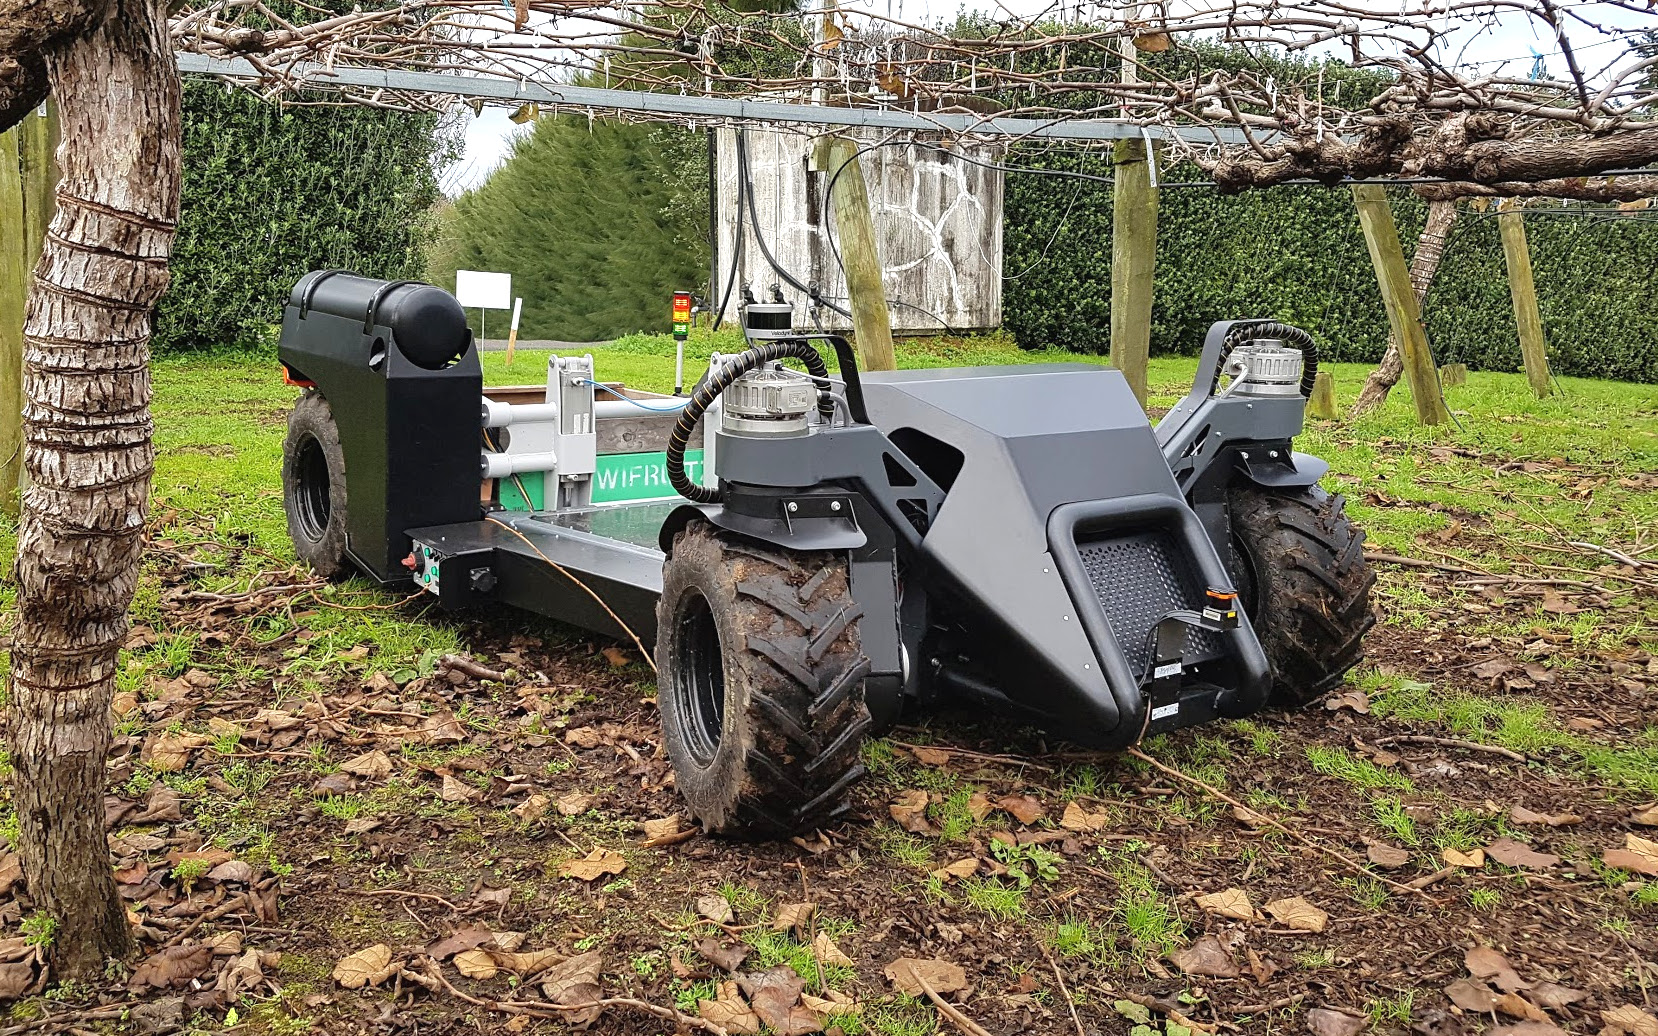
\includegraphics[width=\linewidth]{imgs/photos/suzy_general.jpg}
        % 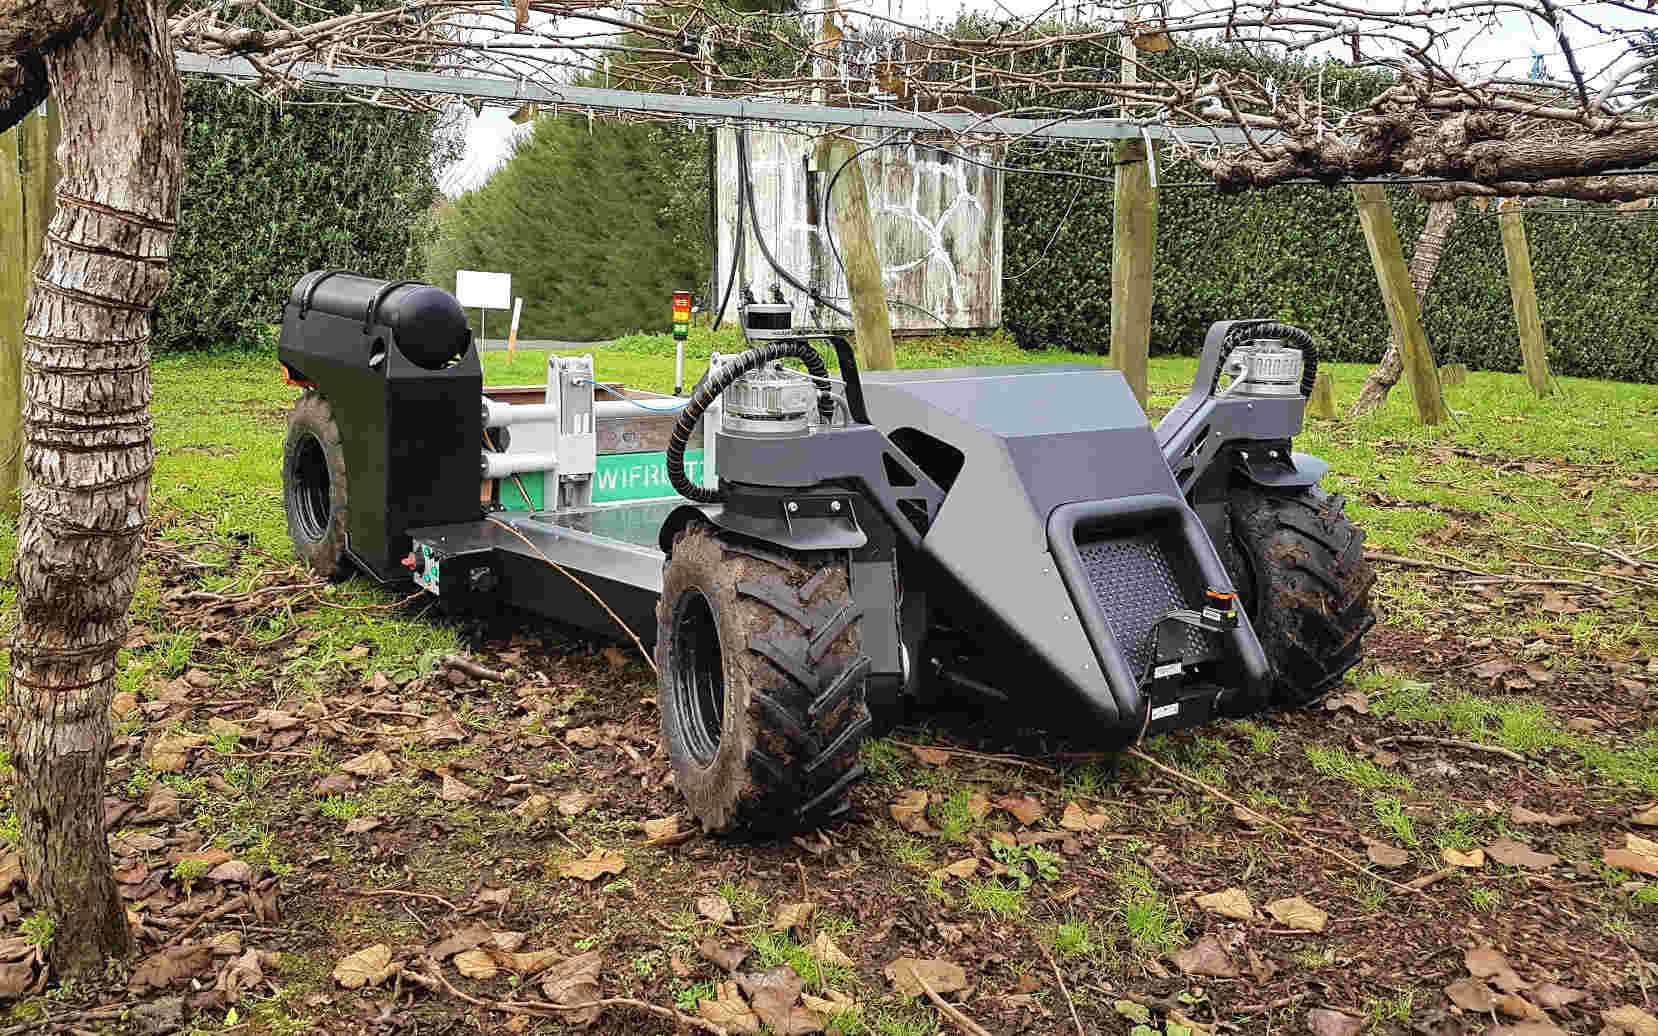
\includegraphics[width=\linewidth]{imgs/photos/suzy_general_small.jpg}
        \caption{
            The platform driving through a pergola style kiwifruit orchard.
        }
        \label{fig:suzy}
    \end{figure}


\section{Related Work}
\label{sect:review}

    \subsection{Purpose-built Autonomous Vehicles in Agriculture}

        The introduction of computers and digital camera technology during the 1980s sparked research into autonomous vehicles for agricultural use \citep{Li2009}.
        When publishing details of an autonomous vehicle in 1998, Tillett et~al.\@ cite difficulties dealing with variability in lighting and the environment as the reason no commercial vehicles were available at the time \citep{Tillett1998}.
        Their vehicle combined wheel encoders, a compass, and accelerometers for odometry information.
        It also featured a camera based row guidance system.
        The system as a whole was capable of spraying individual plants whilst driving autonomously at \SI{0.7}{\meter\per\second} (\SI{2.5}{\kilo\meter\per\hour}).
        % While their purpose built experimental vehicle proved capable of row following and targeted spraying, it was not designed as a modular unit for carrying heavy payloads.
        While their purpose built experimental vehicle proved capable of row following and targeted spraying, it was not designed as a modular unit.


        % It was capable of spraying individual plants whilst autonomously driving at \SI{0.69}{\meter\per\second} (\SI{2.5}{\kilo\meter\per\hour}).


        Four years later, two autonomous vehicles designed for weed mapping and control in open field crops were presented \citep{Pedersen2002,Astrand2002}.
        These platforms had relatively simple chassis and drive systems as they were both at a prototype stage, i.e., neither were designed to carry heavy payloads.
        The first vehicle, presented by Åstrand \& Baerveldt, featured two wheel steering, was two wheel drive, had a camera based row guidance system, was fitted with batteries plus a combustion engine, and an air compressor.
        While its appearance resembles that of a computer server rack on wheels, it contained much of the functionality required of a platform for kiwifruit harvesting and pollination modules.
        The second unit, described by Pedersen et~al.\@, was four wheel drive with two wheel steering and used GPS as its primary navigation sensor.
        It was battery powered only and lacked any sort of row guidance sensor or power generation unit.
        The authors found that row-crop based navigation from GPS alone was not practical and proposed the integration of a row guidance sensor in their next design.
        They also proposed a revised drive system with four wheel steering and a Controller Area Network (CAN) bus for low-level system communication as opposed to using serial links.


        % Both featured two-wheel steering and were designed specifically for field crops.
        % While both were battery powered, the platform presented by \cite{Astrand2002} could also be fitted with a combustion engine.
        % The vehicle presented by \cite{Pedersen2002} was designed to follow pre-defined GPS based paths through row crops, but the authors found that this was impractical without a dedicated row guidance sensor.
        % They proposed a revised design that featured a row guidance sensor, a revised drive system with four-wheel steering, and a Controller Area Network (CAN) bus for low-level communication.

        % Two years later, the revised design proposed by \cite{Pedersen2002} was presented by \cite{Bak2004}.
        The revised design proposed by \cite{Pedersen2002} was presented two years later by \cite{Bak2004}.
        The drive system was modularised with four identical drive/steering modules mounted to the chassis for locomotion.
        The revised chassis featured a three-point suspension system that ensured all four wheels stayed in contact with the ground.
        % The GPS receiver on this platform utilised Real Time Kinematic (RTK) corrections from a base station.
        % The use of a fibe-optic gyro, compass, and wheel encoders meant that accurate localisation was still possible in the event of GPS drop-out.
        The system also incorporated the row guidance sensor as proposed in earlier work, as well as a Real-Time Kinematic enabled GPS receiver, fiber-optic gyro, compass, and wheel encoders.
        The authors noted that the control strategy for the four independently controlled wheels was non-trivial.
        While much more developed than the previous work of \citep{Pedersen2002}, the platform was not designed to: carry heavy payloads, operate in the absence of satellite navigation, or power itself beyond its battery capacity.
        Being designed for row-crops, the chassis sits relatively high from the ground with its payload sensors inspecting the ground below.
        % RTK-GPS is capable of providing positioning with accuracies of \SI{2}{\centi\meter}.


        In 2009, details of BoniRob were published by \cite{Ruckelshausen2009}.
        Similar to the previous unit presented by \cite{Bak2004}, it featured a gyroscope, RTK-GPS for localisation, a CAN bus for communication, and four-wheel steering.
        What made BoniRob particularly interesting is its ability to alter its track width by actuating the arms to which its wheels were attached.
        A \SI{2.8}{\kilo\watt} petrol generator could be mounted to the chassis, additional to its on-board batteries.
        It was capable of carrying a \SI{150}{\kilo\gram} payload in its dedicated module space, which happens to be the gross weight of the vehicle presented by \cite{Bak2004}.
        It introduced the use of both single-plane and multi-layer laser range scanning, known as lidar, for perception and row detection.
        Like the robots before it, BoniRob was designed for use on open field crops.
        During the previous year, some of these authors published details of a much simpler robot named `Weedy' \citep{Klose2008}, also an open field crop based sensing platform.
        BoniRob represents the first of the more general purpose platforms designed to carry modularised payloads, albeit with limited capacity.

        Of particular relevance to this work is that of Scarfe et~al.\@ on an autonomous kiwifruit picking robot \citep{scarfe2009, Scarfe2012}.
        That work involved the creation of a hydraulically driven platform, with two-wheel steering and four wheel drive, to which four fruit harvesting arms were integrated.
        While that platform was designed to navigate kiwifruit orchards autonomously, its ability to do so was not tested due to an outbreak of \textit{Pseudomonas syringae pv. actinidiae} (PSA) that closed access to kiwifruit orchards.
        The platform had a petrol engine for on-board power generation and made use of camera and lidar based row guidance sensors.
        It was low slung and had sufficient carrying capacity, however it lacked the modularity of a general purpose platform, meaning it could only ever be used to harvest kiwifruit.


        Most recently, \cite{Bawden2017} presented their field crop robot - Agbot~II.
        For traction it uses two driven wheels in a differential drive configuration, with two castor wheels for support.
        It is battery powered and designed to autonomously return to a shipping container with a in-built solar powered charging station.
        Their platform is comprised of two side modules bridged by a modular centrepiece containing instrumentation.
        The side modules contain the drive system, whereas the centrepiece is specific to the application.
        The choice of a differential drive system has considerably reduced the robot's complexity and weight over other designs, such as those previously discussed.
        The platform is over \SI{3}{\meter} in width, making it unsuitable for turning between rows of a kiwifruit orchard.
        Hovever, the modularity of the chassis should facilitate easy modification to reduce the total width.
        With a lack of on-board power generation and no means of carrying a fruit bin or a \SI{1000}{\kilo\gram} payload, the design does not meet the requirements for use in kiwifruit orchards.

        A trend with the platforms reviewed, all of which were designed for open field crops, was the favoring of four-wheeled over two-wheeled steering, with the exception of the Agbot II.
        The maneuverability offered by this configuration is not deemed necessary in kiwifruit orchards as headland areas are large enough for tractors to maneuver.
        Only the platform of \cite{Scarfe2012} had the capacity for carrying fruit bins.

        % Finally, to aid development, the use of open source simulation tools allowed the creators of BoniRob to develop and test their mobility system independent from the physical hardware.

        \cite{Blackmore2007} envisaged significant reductions in production costs for agricultural robotics by repurposing parts already in use in the agricultural and automotive industry.
        While not a physical component, the CAN bus is one such technology borrowed from these industries.
        Most of the more recent platforms reviewed made use of this communication system.

    \subsection{Sensors for Row Based Navigation in Orchards}

        Since the vehicle is designed for autonomy, selecting appropriate sensors and developing the vehicle around these sensors is an important design consideration.
        Sensor combinations for orchard based row detection mostly fall into three categories; camera based, lidar based, or a combination of the two.
        The following section summarises a review of row detection efforts in orchards using these techniques.

        % Lidar come in two flavours: single-plane, and multi-layer.

        \cite{Subramanian2006} tested both camera and lidar (Sick LMS-200) based guidance systems in a citrus fruit orchard.
        Sensors were trialled separately on a tractor retrofitted with a drive-by-wire system.
        Their vehicle was able to navigate a small and simplified path using both machine vision and lidar based approaches at speeds of up to \SI{4.4}{\meter\per\second} (\SI{15}{\kilo\meter\per\hour}).
        They found that lidar proved more accurate until the lidar's data transfer rate became a limiting factor.
        The 2D camera based approach was favorable after this point.
        They suggest that combining the two systems would give more robust guidance as well as providing the ability to detect obstacles.
        No mention of the ability for the image based approach to cope with varying lighting conditions is made.
        These results are promising for use in kiwifruit orchards, where the conditions are similar and where the target operating speed is only \SI{1.39}{\meter\per\second} (\SI{5.0}{\kilo\meter\per\hour}).

        \cite{Barawid2007} demonstrate the use of data from a single-plane lidar (Sick LMS-219) to guide a drive-by-wire tractor through an orchard.
        Their results show real-time processing of lidar data is sufficient to navigate an orchard at \SI{0.36}{\meter\per\second} (\SI{1.3}{\kilo\meter\per\hour}).

        In 2011, two groups published work on the generation of centre lines from camera data taken in orchard rows.
        \cite{He2011} uses traditional machine vision, where \cite{Torres2011} makes use of neural network based image processing.
        Both methods generated valid paths, although He et~al.\@ note that theirs may not be suitable when the environment background becomes complex.
        The neural network based approach of \cite{Torres2011} appeared to cope better with variations in lighting and row spacing.
        Also in 2011, \cite{Hansen2011} showed the use of a single-plane lidar (Sick LMS-200) for vehicle localisation in an orchard.

        The work of \cite{Scarfe2012}, combined traditional camera based image processing techniques with a single-plane lidar (Sick LMS-111).
        The image based approach failed to cope with variability in lighting conditions, however the lidar proved useful for detecting the trunks and posts in kiwifruit orchards.

        \cite{Freitas2012} focused on the detection of people and bins within rows of an apple orchard using lidar (Sick LMS-291), a low-cost inertial measurement unit, and wheel encoders.
        Their algorithm was capable of detecting each obstacle class off-line using data captured from a test orchard.

        \cite{Zhang2014} used a lidar (Hokuyo UTM-30LX) to generate maps of an apple orchard with the aid of artificial landmarks.
        They used an actuated single-plane lidar to generate multi-plane data for use in row and landmark based sensing.
        Placing artificial land-marks in orchards was intended to reduce the effort required to create orchard maps for guidance systems.

        The following year, many of the same authors from  the paper presented by \cite{Zhang2014} write about their autonomous vehicle \citep{Bergerman2015}.
        It describes an electric utility vehicle converted to drive-by-wire with the addition wheel encoders for odometry and a single-plane lidar (Sick LMS-111).
        While not demonstrated detecting obstacles in real-time, their previous work processing off-line data \citep{Freitas2012} has potential to be integrated on their platform with the addition of extra computing power.

        Most recently, \cite{Sharifi2015} write about a method to generate centre-lines from 2D images of orchard rows.
        Like the work of \cite{He2011}, the technique offers a way to generate paths from a single camera image without resorting to neural networks.
        However, their future work focuses on increasing robustness to variations in lighting conditions, which indicates issues in this area.
        They state their system has use in being complementary to lidar based navigation.

        The experiences of \cite{Scarfe2012}, and others, indicate that a lidar outputs data that requires less post-processing to be robust.
        The use of lidar has seen two of the reported vehicles navigate autonomously through orchard environments, which is encouraging.
        Other reports suggest that traditional image based processing for navigation fails when the scene becomes complex or significant variations in lighting occur.
        Combining cameras with neural network based processing increases the robustness to environmental complexities, such as light or clutter, at the expense of increased computation resources.
        % Common among these vehicles is the use of sensor fusion, whereby data from multiple sensors is merged and filtered.
        % This provides a way to combine the advantages of multiple sensor types, and the benefit of redundancy  into a single computation space.

        With regards to the use of RTK-GPS in guidance systems, Slaughter et~al.\@ points out the trade-off of requiring an ``unobstructed `view' of the sky from all parts of the field'' \citep{Slaughter2008}.
        % Additionally, multi-path signal propagation caused by nearby foliage or the geometry of the land itself presents its own mode of failure \citep{Durrant-Whyte2005}.
        % A feasibility analysis by \cite{Pedersen2006} highlighted the use of RTK-GPS systems as a significant cost in yearly subscriptions alone.
        \cite{Durrant-Whyte2005} describe one failure mode of GPS being multi-path signal propagation caused by nearby foliage or the geometry of the land itself.
        % This requirement can not be satisfied under the canopy of a kiwifruit orchard which are usually surrounded by tall wind-breaking hedges.
        % \cite{Torii2000} suggests a combination of both RTK-GPS and machine vision systems to be the most promising system going forward based on reductions in costs and increases in performance of these systems.
        % While \cite{Li2009} concludes that either GPS and machine vision, or GPS and lidar will be used together as a development trend.
        \cite{Li2009} conclude that the use of either GPS and machine vision, or GPS and lidar will become a development trend.
        Based on the increased reception requirements, we discount the use of an RTK-GPS system, but still consider the use of GPS in-orchard.

\section{Platform Design}
\label{sect:design}
    % \subsection{Vehicle Configuration}
    % \label{sect:mechanical}

        \begin{figure}[htb]
        \centering
        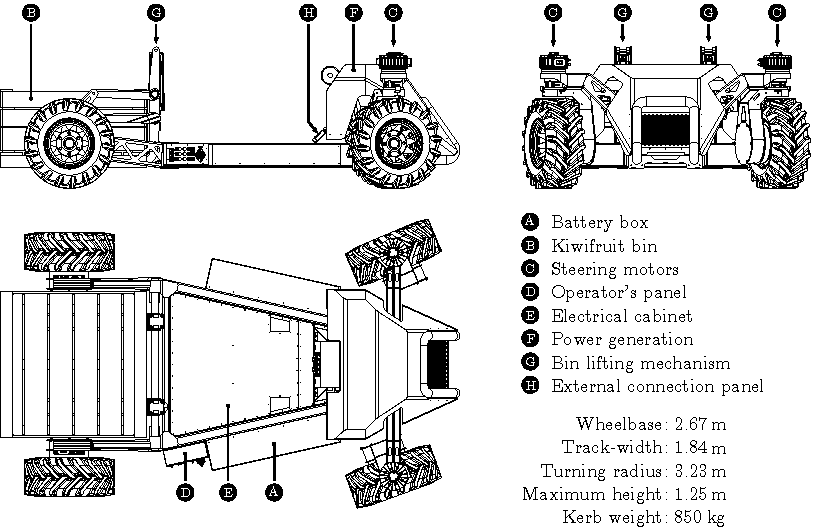
\includegraphics[width=\linewidth]{imgs/profile_views/AMMP-All-Labelled.pdf}
        \caption{Profile drawings of the robotic platform with kiwifruit bin.}
        \label{fig:AMMP}
        \end{figure}

        The vehicle's design is mostly influenced by the need to carry robotic modules and fruit bins through pergola style orchards.
        Existing commercial platforms suitable for use in horticulture exist, such as the Warthog from ClearPath Robotics, but the maximum payload, battey life, and vehicle geometry make it and similar offerings unsuitable.
        Robotic modules for pollination or harvesting can weigh as much as \SI{600}{\kilo\gram} and a bin of kiwifruit adds an additional \SI{400}{\kilo\gram}.
        The canopy height in these orchards ranges from \SI{1.4}{\meter} to \SI{1.7}{\meter} so the vehicle must have a low profile.
        Modules carried by the platform require clearance from the canopy in addition to the height they occupy themselves.
        To maximise the space available to these modules the platform must be low-slung at the point they attach.
        Figure \ref{fig:AMMP} illustrates the platform's design, with module area allocated between markers `G' and `H' in the side view (top left).
        The top surface of the chassis in this region sits \SI{360}{\milli\meter} above the ground.

        The chassis is assembled from sections of \SI{3}{\milli\meter} laser-cut and folded mild-steel.
        The sections are welded together on jigs, also made from laser-cut and folded steel, before being powder coated.
        Finite element analysis was used during the design phase to help identify areas needing to be strengthened and areas where material could be removed.
        Much of the folded chassis structure contains triangular cut-outs, which reduces weight and has minimal impact on rigidity.
        This helped to ensure the platform meets its target load capacity of \SI{1000}{\kilo\gram}, while the structural chassis weighs only \SI{200}{\kilo\gram} \color{red}Validate this figure in SolidWorks\color{black}.
        Bin lifting forks sit in the area between the rear wheels.
        The lifter is actuated by two vertically mounted pneumatic cylinders and is controlled by a standard pneumatic valve block.
        Fuel and compressed air tanks sit over the right-hand rear wheel, while not shown in figure \ref{fig:AMMP} they can be seen in figure \ref{fig:suzy}.

    \subsection{Steering}
    \label{sub:steering}

        The angles of the vehicle's front wheels are actuated independently following the Ackermann steering geometry principle.
        Actuation is performed by brushless AC motors (Heinzmann PSM G100) mounted vertically above each drive wheel.
        These motors can generate \SI{7.32}{\newton\meter} of torque with a maximum angular velocity of \SI{3000}{rev\per\minute} and are rated at \SI{2.3}{\kilo\watt}.
        The outputs are fed through fixed-ratio planetary gearboxes with a 64:1 reduction, increasing torque to \SI{470}{\newton\meter} while reducing the maximum angular velocity to \SI{47}{rev\per\min}.

        Torque requirements for the front steering motors were calculated as:
        \begin{equation}
        \label{eqn:steer_torque}
        \tau = W u \sqrt{\frac{B^2}{8} + E^2}
        \end{equation}
        where $\tau$ is the required static torque, $W$ is the force transmitted through the wheel, $u$ is the coefficient of friction, $B$ is the nominal width of the tyre, and $E$ is the offset between the tyre's contact surface and its axis of rotation.
        The axis of rotation on this vehicle lies directly through the centre of the wheel, meaning $E=0$.
        % As the axis of steering rotation lies directly through the centre of the wheel, $E=0$.
        A value of 0.75 was used as the coefficient of friction as a best guess representation of a tractor-grip tyre on dry concrete.
        The weight of the vehicle (\SI{800}{\kilo\gram}), plus payload (\SI{1000}{\kilo\gram}), and fuel (\SI{60}{\kilo\gram}) gives a total mass of \SI{1860}{\kilo\gram}.
        Allowing for uneven weight distribution on the vehicle and a safety margin, the per wheel mass supported is \SI{500}{\kilo\gram} giving a weight of \SI{4900}{\newton}.
        The width of the tyres is \SI{0.28}{\meter}.
        Combining these values in Equation~\ref{eqn:steer_torque} yields a required torque of \SI{388}{\newton} to overcome static friction.

        Actuating the wheels independently removes the need for mechanical linkages between them allowing for more extreme steering angles and a simpler mechanical design.
        Both steered wheels have the freedom to rotate \SI{330}{\degree}, artificially limited by mechanical stops.
        At its most extreme steering angle the centre-point of the turn is located at the midpoint of the rear wheels.
        During such a turn the turning radius is approximately equal to the vehicle's wheelbase.
        This sees the vehicle turn between orchard rows spaced as little as \SI{3}{\meter} apart.
        % It is often possible for the vehicle to make a \SI{180}{\degree} turn mid-row, something not possible for most commercial vehicles designed for orchard use.
        % This range in steering angle allows the vehicle to place the centre of rotation at the mid-point between its rear wheels during its tightest turn.
        % At this steering angle, .
        Implementing four-wheel steering system would shift the pivot point to the vehicle's centre, roughly halving the radius.
        This is unnecessary as headlands in kiwifruit orchards are sized for tractors with much larger turning radii than the developed platform.
        The two wheeled steering system removes the need to develop the ``non-trivial'' control strategies encoutered by \cite{Bak2004}.
        It also increases the usable area at the rear of the vehicle by removing the need for clearances around actuated wheels.
        A differential drive, or skid steer, system was expected to cause ground damage to a level considered unacceptable to orchard owners when carrying heavy loads.

        \color{red} Add a drawing here of the proxy ring\color{black}
        The steering motors have incremental encoders, but no means of absolute positioning built-in.
        This means the front wheels must alighed during a homing sequence at boot-up to find an absolute angle to reference from.
        Proxy sensors are used as a means of aligning the front wheels during the homing sequence.

    \subsection{Drive system}
    \label{sub:drive}

        The platform has no suspension other than what is provided by its tyres.
        As the intended operating speed within an orchard is \SI{5}{\kilo\meter\per\hour}, a dedicated suspension system is not deemed necessary.
        A front pivoting axle ensures that all four wheels remain in contact with the ground.
        \color{red} Drawing of front pivoting axel\color{black}

        Estimation of the required torque is calculated by the following equations:
        \begin{align}
        \label{eqn_f_rolling}
        F_{rolling} &= C_{rr} \times m\\
        F_{grade} &= m \times G \times \sin(\alpha)\\
        F_{accel} &= m \frac{\Delta v}{t}\\
        \label{eqn_f_accel}
        F_{total} &= F_{rolling} + F_{grade} + F_{accel}
        \end{align}
        Where $F_{rolling}$ is the force due to rolling resistance; $F_{grade}$ is the a grade resistance force; and $F_{accel}$ is the force required to accelerate forward.
        A rolling resistance coefficient ($C_{rr}$) of 0.04 was chosen based on values found in automotive handbooks.
        It represents the case of a pneumatic tyre on medium-hard soil.
        Other variables used are: a vehicle mass ($m$) of \SI{1900}{\kilo\gram}, slope angle ($\alpha$) of \SI{20}{\degree}, velocity change ($\Delta t$) of \SI{2.78}{\metre\per\second} (\SI{10}{\kilo\meter\per\hour}), and an acceleration time ($t$) of \SI{6}{\second}.
        Putting these values through Equations \ref{eqn_f_rolling}--\ref{eqn_f_accel} gives a total force requirement of \SI{7.99}{\kilo\newton}.
        On a per wheel basis this is \SI{2.0}{\kilo\newton}, or \SI{729}{\newton\meter} when taking the wheel radius ($r$) of \SI{0.365}{\meter} into account.
        Required traction power ($P$) was then calculated as follows:
        \begin{align}
        \label{eqn_f_power}
        \omega &= 2 \pi \times \frac{v}{2 \pi r} = \frac{v}{r}\\
        P &= \tau \omega
        \end{align}
        where $\omega$ is the angular velocity of a wheel, $v$ is the vehicle velocity, and $\tau$ is torque.
        At a velocity of \SI{2.78}{\meter\per\second} (\SI{10}{\kilo\meter\per\hour}), the calculations give a power requirement of \SI{5.55}{\kilo\watt} per wheel.

        The selected motors are hub-mount permanent magnet brushless AC motors with integrated 40:1 fixed-radio plaentary gearboxes (Heinzmann PSM-G120).
        Each motor is rated for \SI{6.4}{\kilo\watt} at \SI{96}{\volt} with a maximum speed of \SI{3000}{rev\per\min} and a torque of \SI{20.4}{\newton\meter}.
        At the output of the gearbox, the torque jumps to \SI{816}{\newton\meter} while the angular velocity drops to \SI{75}{rev\per\minute}.
        This gives the platform a top speed of \SI{10.3}{\kilo\meter\per\hour}.

        % Relevant references are \citep{Bosch2002} and \cite{Wong2001}.
        % A rolling resistance coefficient $C_{rr}$ of 0.04 chosen based on values from various automotive handbooks \citep{Bosch2002}.

        In total there are seven brushless AC motors on-board the platform: four drive motors, two steering motors, and a motor used for electrical power generation.
        Each are connected to separate, but identical, AC motor controllers (Sevcon Gen4 Size 4).
        These controllers are available in four bus voltage options: 24-36V, 36-48V, 72V-80V, and 96V-110V.
        The six motors used for traction and steering are together capable of consuming \SI{30.2}{\kilo\watt}.
        Using a \SI{48}{\volt}DC bus, this would equate to a current draw of \SI{630}{\ampere}.
        As approximately \SI{20}{\meter} of cabling is required to connect the motors and controllers to a common point on the vehicle, a \SI{96}{\volt}DC bus was used to reduce the required gauge of that cable.


    \subsection{Power Distribution}
    \label{sub:power}
        The system bus connects the batteries and generator to motor controllers and on-board power converters.
        A series of heavy-duty contactors (TE Connectivity LEV200 Kilovac) control each device's connection to the bus, as well as the bus's connection to a power source.
        Figure \ref{fig:power_system_diagram} illustrates how in which each component is connected.

        \begin{figure}[htb]
            \centering
            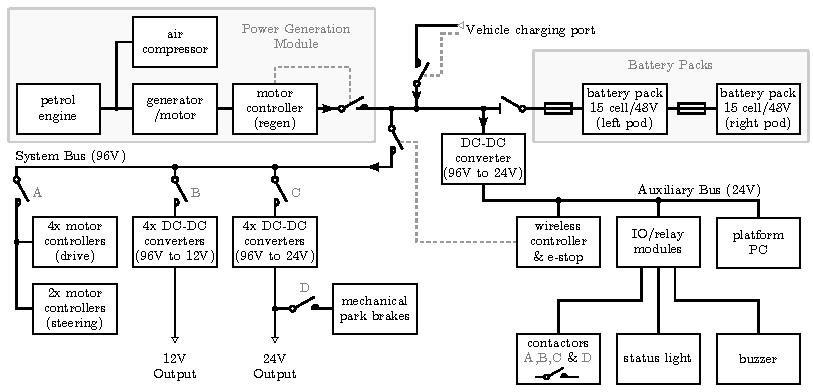
\includegraphics[width=\linewidth]{imgs/system_diagram/full-system-diagram_v1.pdf}
            \caption{Power distribution system diagram. Dashed lines in grey indicate control lines to contactors.
                     The system is a series hybrid configuraton with respect to the engine and battery pack.}
            \label{fig:power_system_diagram}
        \end{figure}

        Two battery modules attached to the sides of the chassis each house fifteen lithium-iron-phosphate (LiFePO$_{\text{4}}$) batteries connected in series.
        Together, the batteries (Winston/Thundersky WB-LYP90AHA) provide a nominal bus voltage of \SI{96}{\volt} and a total electrical capacity of \SI{8.64}{\kilo\watt\hour}.
        The battery packs were `bottom-balanced' before being fitted and no cell-level voltage monitoring is present.
        Maximum and minimum pack voltages were established by monitoring individual cells during charging and discharging.
        At the point that any individual cell exceeds a safe maximum/minimum threshold, the respective maximum/minimum pack voltage is recorded at that point.
        A hermetically sealed disconnect switch (Gigivac HBD41) separates the batteries from the system.
        Once closed, an auxiliary 24V bus becomes powered that powers componenets required to start the rest of the rest of the system, including the generator.

        A power generation unit comprised of a petrol engine (Honda GX-690), air compressor (Rotorcomp NK-1), and electrical generator (Heinzmann PMSG-150) sits over the front pivoting axle.
        The drive shafts of the three units are connected via pullies and a heavy-duty timing belt.
        The engine, compressor, and alternator can be controlled and monitored by microcontroller based control board.
        This board connects to the Platform PC via the platform's CAN bus.
        The engine is capable of producing \SI{16}{\kilo\watt}, where up to \SI{9.6}{\kilo\watt} is converted to electrical power and \SI{4.0}{\kilo\watt} to pneunatic power.

        Electrical energy from the power generation unit is fed to the battery modules in a series-hybrid configuration.
        An external charging port is also fitted to allow charging of the batteries without using the petrol engine.

        The fuel tank can hold approximately \SI{60}{\litre} of petrol, providing enough energy to operate for approximately \SI{24}{\hour}.
        On-board DC-DC converters can continuously deliver \SI{2.8}{\kilo\watt} at \SI{12}{\volt}DC, \SI{3.8}{\kilo\watt} at \SI{24}{\volt}DC, and \SI{3.5}{\kilo\watt} at \SI{240}{\volt}AC, simultaneously.
        A connection panel near the front of the platform houses the weather-sealed plugs through which these outputs are accessible.


    \subsection{Communications Architecture}
    \label{sect:architecture}

        \begin{figure}[htb]
            \centering
            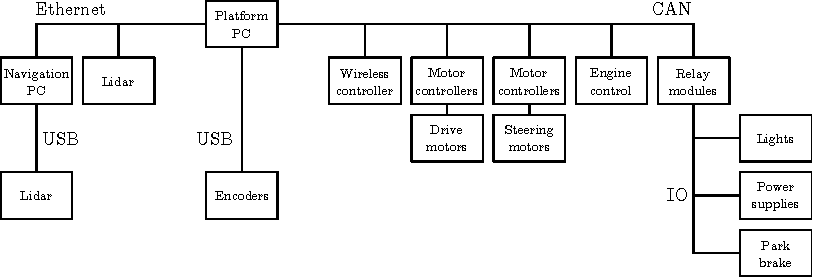
\includegraphics[width=\linewidth]{imgs/system_diagram/diagram_v4.pdf}
            \caption{Communications level system diagram showing the types of interfaces and relative relations on the platform.}
            \label{fig:system_diagram}
        \end{figure}

        % This section briefly explains the hardware and software architecture of the platform.
        Standardised protocols and software frameworks are employed where possible, supplemented with custom solutions only when needed.
        The platform is centrally controlled by an x86 based small-form-factor PC (Intel NUC) running Ubuntu 16.04 server edition.
        This computer is connected to an on-board Ethernet network and CAN bus via a USB-to-serial CAN adaptor (IXXAT USB-to-CAN v2).
        Figure \ref{fig:system_diagram} shows a simplified arrangement of connections between each devices.
        Low-level hardware devices on the platform, such as motor controllers and relays, are connected to the Platform PC via CAN bus.

        An Ethernet network connects the Platform PC to a second computer dedicated to task of autonomous navigation.
        It too is an x86 based PC running Ubuntu, but uses a microATX form-factor motherboard with a discrete graphics card (Nvidia GTX 1080).
        This PC is responsible for autonomous navigation tasks, such as connecting to sensors, filtering and processing data, and sending drive commands to the Platform PC.
        The graphics card is used to accelerate neural network algorithms and some image processing functions.

        The open source Robotic Operating System (ROS) is used to facilitate communication between both computers and between software nodes within each machine.
        Figure \ref{fig:system_diagram_software} shows a simplified passage of information flowing through the navigation system.
        To maximise code reusablility, each device on the platform has its own ROS node dedicated to publishing device data or subscribing to generated device commands.
        Interface adapters, motor controllers, wireless controllers, lidar, and encoders are such devices with dedicated interface nodes.
        Nodes are also used to transform or perform calculations on data and pass it between nodes written in either C++ or Python.
        For instance, as shown in figure \ref{fig:system_diagram_software}, an `Ackermann kinematics' node transforms steering input data into individual wheel velocity and position/angle outputs.
        This node could easily be swapped out for a different translator node during run-time without disturbing the system.

        In a starndard configuration, the motor controllers are interfaced using a combination of analog and digital inputs.
        For example, the accelerator and steering inputs are set by potentiometers actuated by the vehicle's driver.
        However, the controllers also provide an option for a multi-motor vehicle configuration.
        In this configuration, inputs fed into a master controller are relayed to a second controller over a CAN interface.
        By observing the communication protocol between a master and slave in operation, it was possible to implement a master node in software that runs on the Platform PC.
        With this, all motor controllers on the platform are programmed as slave devices.
        This forces them to accept drive commands via their CAN interafce which are generated from ROS nodes on the Platform PC.

        Relay modules allow the Platform PC to toggle power to on-board power supplies, motor controllers, park-brakes, and lights.
        These modules also monitor the timing of synchronisation messages transmitted by the Platform PC onto the CAN bus, which should occur every \SI{20}{\milli\second}.
        Once a module detects an absence of synchronisation messages for \SI{100}{\milli\second} or longer it enters a defined error state.
        % If the module does not receive a syncronisation message for \SI{100}{\milli\second} it will enter an error state.
        That state will result in the motor controllers and on-board power supplies being shut-off and the park brakes engaged.
        Since power is required to disengage the park brakes, this equates to `shutting-off' the brake release mechanism.
        CAN bus monitoring ensures that the system is automatically shut down should the Platform PC become unresponsive.


        \begin{figure}[htb]
            \centering
            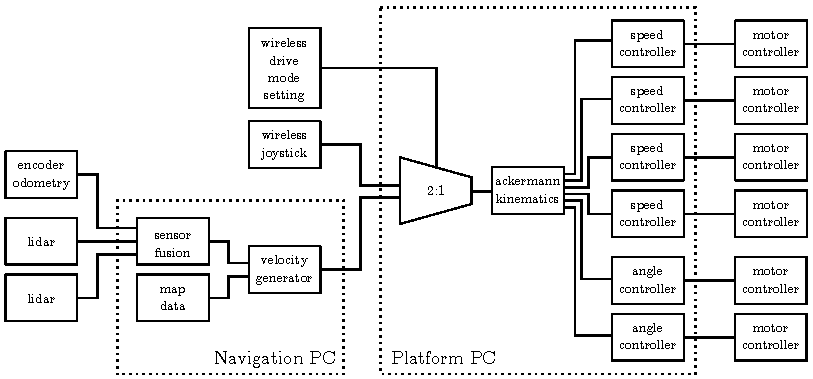
\includegraphics[width=\linewidth]{imgs/system_diagram/software_v2.pdf}
            \caption{Simplified system diagram (partial) showing node connectivity used for manual and autonomous platform control.}
            \label{fig:system_diagram_software}
        \end{figure}

        In addition to the drive commands generated by the navigation system, a safety rated wireless controller (HBC Radiomatic Eco) lets the operator issue drive commands via joystick.
        The joystick also has a mode switch that allows the operator to select between manual and autonomous control, and an emergency stop button.

    \subsection{Testing}
    \label{sub:drivability_tests}
        Tests of the vehicle's steering and stopping performance as well as its structural integrity was carried out.
        In each situation a \SI{1100}{\kilo\gram} mass was strapped to the module area.
        No deflection of the vehicle's chassis was evident upon application of the test mass.
        Deflection of between 1 and \SI{2}{\milli\meter} was measured between the front pivot and the wheel supports.
        Static steering tests conducted on a dry concrete surface showed no reduction in ability to turn under these conditions.
        Dynamic tests involved three instances of stopping whilst driving down a \SI{10}{\degree} slope.
        During each test the vehicle came to a complete stop within a distance of \SI{2.4}{\meter}.


    \subsection{Discussion}
    \label{sub:discussion}

        The \SI{96}{\volt} battery pack introduced an electrical hazard that required risk mitigation procedures to be followed when working on the unit.
        While essential for safety, these procedures added complexities and delays during which could have been avoided by adopting a lower pack voltage.
        The authors suggest a pack voltage of \SI{48}{\volt} as a safer alternative during vehicle development as it bears a reduced risk of injury from electric shock.
        Inputs of \SI{48}{\volt} are supported across a wider range of motors, motor controllers, and power converters, but cabling requirements are increased.

        The series hybrid configuration allows the vehicle to drive and provide power to subsystems without the petrol engine.
        This is useful in testing scenarios, where people are in close proximity to the vehicle, as it eliminates exhaust fumes and reduces both noise and vibration.
        However, robotic modules and the bin lifting mechanism require pneumatic air pressure to operate.
        As the air compressor is belt driven from the petrol engine, it is necessary to frequently run the engine to provide air to these systems.
        An electric air compressor would allow for the system unassisted by the petrol engine for much longer periods.

\section{Navigation Sensors}
\label{sect:sensors}
    The choice of sensors incorporated into a vehicle determines which algorithmic approaches are available for navigation and object detection.
    This section investigates the use of lidar, GNSS receivers, and cameras in-orchard.
    Following this, each sensor's ability to capture relevant data is tested.
    Finally, the performance of appropriate sensors with prototype navigation and object detection algorithms is presented.
    Evaluations of each sensor is discussed in the context of orchard based navigation.

\subsection{Sensor Selection}

    As the drive motors have built-in wheel encoders, basic odometry data is already available.
    Encoders on driven wheels will give false readings if wheel slip occurs so should not be used for odomentry alone.
    However, the data they provide can be used to assist with mapping, localisation, and provide velocity feedback.

    Other sensors considered for inclusion are outlined in Table \ref{table:sensor_comparison} with their associated issues.
    Factors considered were strengths and weaknesses in the context of orchard use, reported usage in literature, and availability at a suitable price.
    The investigation highlighted both lidar and 2D cameras as offering high functionality for navigation and object detection.
    Time-of-flight cameras were a compelling option based on a cost-benefit analysis; especially if cheaper units work in sunlight.
    Because localisation is such a key function, the performance of two GNSS receivers have also been evaluated.
    % The following sections detail our experiences while trialling these sensors.
    \begin{table}[htbp]
        \centering
        \footnotesize
        \begin{tabular}{ l l}

            \textbf{Sensor Type}      &\textbf{Common Issues} \\ \hline
            GNSS receiver              & Prone to signal loss from surrounding foliage\\  \hline
            Inertial Measurement Unit & Error accumulation and thermal drift\\ \hline
            Digital Compass           & Prone to disturbance by nearby metallic structures\\ \hline
            Encoder                   & Error accumulation \\ \hline
            Lidar                     & Reduced visibility in fog and heavy rain \\ \hline
            Time of Flight Camera     & Reduced visibility in sunlight, fog and heavy rain \\ \hline
            Camera                    & Reduced visibility in fog or direct sunlight \\ \hline
            Thermal Camera            & Reduced visibility in conditions of low thermal contrast\\ \hline
        \end{tabular}
        \caption{Sensor types considered for inclusion on the platform.}
        \label{table:sensor_comparison}
    \end{table}

% \subsection{Data Collection and Inspection}
 %    The sensors that seemed important to test, based on both the literature survey and the cost-benefit analysis were lidar, cameras and GPS.
	% In addition, time of flight cameras were considered, because they seemed to be a compelling option based on the cost-benefit analysis; especially if some of the less expensive models were found to work well in sunlight.
	% It was also decided that encoders would be tested in favour of using an IMU because the encoders were built into the AMMP motors.
	% Some data was collected from each sensor in order to decide which sensors to prototype algorithms for.

    \subsubsection{In-orchard GNSS Evaluation}
        Two GNSS receivers were evaluated: a Ublox Neo-M8N module and an OmniSTAR 5120VBS with AX0 series antenna.
    	Both were connected to a single board computer (Beaglebone Black) via serial connection for data acquisition.
        The Ublox module was selected for its high sensitivity and internal low-noise amplifier.
        It is capable of receiving GPS, Galileo, GLONASS, and BeiDou GNSS signals concurrently.
        The OmniSTAR receiver was chosen for its external high-gain antenna (34 dB) which claims multi-path rejection.
        It is capable of receiving only GPS signals.

        The testing procedure first involved planning a path through a single row of a kiwifruit orchard and plotting this on a satellite map.
        Waypoints were placed along the row at the location of posts used to hold the canopy's structure.
        Relative distances between these waypoints were measured with a tape measure and recorded.
        The receivers were then tested separately over the course of approximately two hours.
        Before testing, each unit was powered up and given \SI{30}{\minute} to initialise in an open area near the kiwifruit orchard.
        During testing, each unit was walked slowly along the pre-determined path with stops at each waypoint to provide time for a positional fix.
        The path was approximately \SI{500}{\meter} in length and took approximately \SI{15}{\minute} to complete, including stops at each waypoint.
        Waypoints were spaced at intervals of \SI{5.5}{\meter} along the row.

        \begin{figure}[htb]
            \centering
            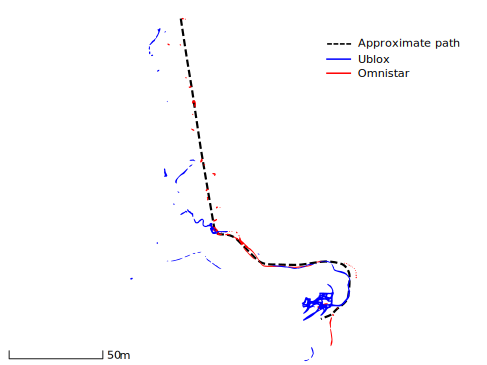
\includegraphics{imgs/gps_path/gps_path.pdf}
            % 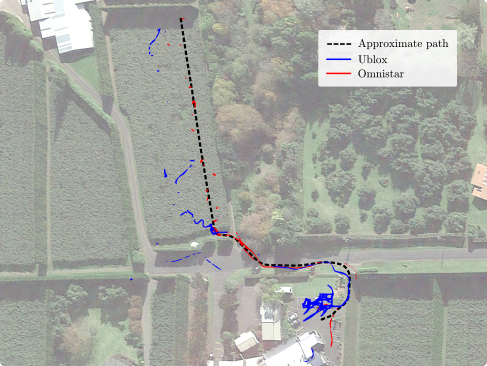
\includegraphics{imgs/gps_path/gps_path_small.png}
            \caption{
                Aerial view of the path taken through the test orchard and the captured GPS data.
            }
            \label{fig:gpsResults}
        \end{figure}

        The path followed, and the corresponding GPS locations collected from the receivers, is presented in figure \ref{fig:gpsResults}.
        It should be noted that data has been recorded for the round-trip so represents two passes along the path.
        It was noticed during testing that the signal quality lights on both GPS receivers regularly indicated a loss of signal.

        The Omnistar receiver appears to track the approximate path well, but the data is sparse with regular loss of signal after entering the orchard.
    	The Ublox receiver collected more data, but was much less accurate.
        It may be possible to use a unit such as the Omnistar, which provided fewer but more accurate readings, as a sanity check for an approximate location within orchards.
        Overall, the units could not be relied on for localisation in this environment.
        These results results, GNSS receivers with similar performance to those trialled are deemed unsuitable for use in kiwifruit orchards.

    \subsubsection{In-orchard Lidar Evaluation}
        Three lidar were evaluated, two single-plane and one multi-layer.
        The two single-plane lidar were the Hokuyo UTM-30LX and a SICK LMS111.
        The multi-layer lidar is a Velodyne VLP-16 which has 16 horizontal \SI{360}{\degree} planes spread over \SI{15}{\degree} vertically.
        Data was collected from each lidar by driving through orchard rows with the sensor placed midway between the ground and canopy (approximately \SI{0.8}{\meter} above the ground).

        \begin{figure}[htb]
            \centering
            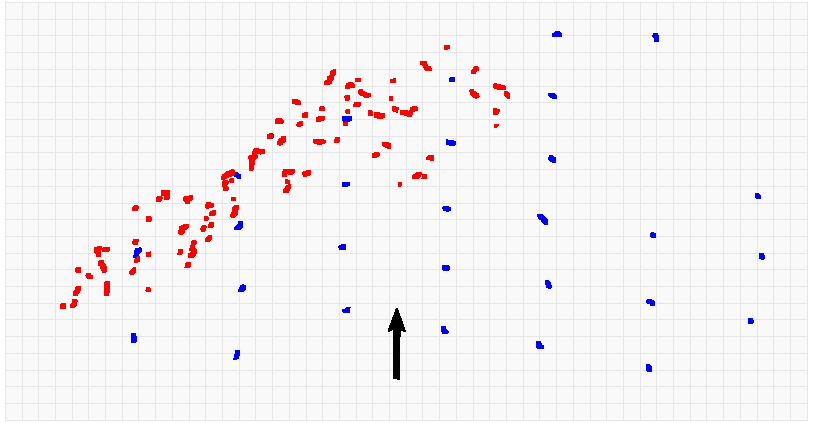
\includegraphics[width=\linewidth]{imgs/canopy_data/canopy_data.pdf}
            \caption{
                Captured lidar data showing the non-structural points reflected by the canopy (indicated by red markers) and structural points from tree trunks and posts (blue markers).
                The arrow indicates the position and heading of the platform at the time of capture.
            }
            \label{fig:canopyDataCloud}
        \end{figure}

        The intention was to use lidar as a means of detecting structure defining features of the orchard, such as posts, trunks and hedges.
        Detecting these features should allow for row boundary detection, or general mapping and localisation.
        However, both single-plane lidar produced clouds of unstructured data amongst the structured features, as shown in figure \ref{fig:canopyDataCloud}.
        This was caused by the lidar's scan plane intercepting with the canopy whilst driving over convex terrain.
        Similarly this issue arose on concave terrain where the plane intercepted with the ground, as depicted in figure \ref{fig:concaveSlope}.

        \begin{figure}[htb]
            \centering
            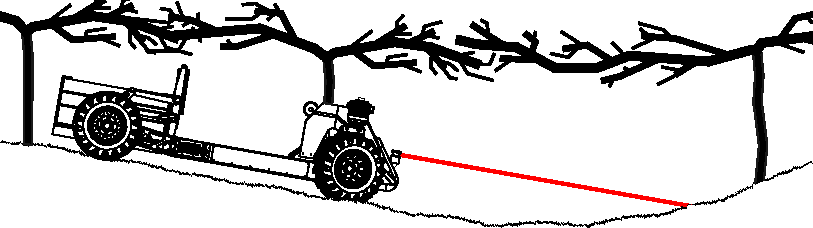
\includegraphics[width=\linewidth]{imgs/concave_slope/concave_slope_v4.pdf}
            \caption{
                On concave slopes the lidar scan plane intercepts with the ground instead of trunks or posts.
                The dashed line shows a horizontal plane coming from the the lidar.
                Dotted lines represent the upper and lower layers taken from the multi-layer lidar.
            }
            \label{fig:concaveSlope}
        \end{figure}

        This issue was reduced by the use of a multi-layer lidar and post-processing.
        Having sixteen layers available meant it was possible to select a scan layer that gives the most useful viewing range.
        Referring to figure \ref{fig:concaveSlope}, that would correspond to the dotted line above the horizontal (dashed) line which intercepts with a row defining feature (a tree trunk).

        It was decided that a multi-layer lidar would be best suited for navigation due to its ability to to see more distant features while driving on undulating ground.
        A single-plane lidar could still be used at short range as an independent channel of processing for redundancy or obstacle detection.
        On our platform, a single-plane lidar was fitted as a detector for possible collisions, and a multi-layer lidar was fitted for navigation use and general object detection.


    \subsubsection{In-orchard Camera Evaluation}
        \label{sect:camera_evaluation}

        Three varieties of camera were tested: time-of-flight, 3D stereoscopic, and traditional 2D cameras.

        The time-of-flight based camera was the Basler TOF640-20GM-850NM.
        It provides range, intensity, and confidence data at a resolution of 640 by 480 pixels.
        This specific model was chosen as it had previously proved useful when collecting depth data of kiwifruit canopies.
        During that time it had been operated under different lighting conditions and exhibited minimal occurrences of data loss.
        However, these navigation based tests revealed that in both direct sunlight and overcast conditions there was significant data loss.

        The 3D stereo camera tested was an Intel RealSense R200.
        It combines a stereo pair of infra-red cameras with a colour camera.
        Additionally, it features an infra-red projector as a means of adding texture to objects in its field of view to assist with stereo processing.
        The appealing characteristics of this sensor were its low cost and its claim of being long-range and able to work outdoors.
        However, in both overcast and sunny conditions it suffered from a complete loss of range data.

        Finally, 2D-cameras were trialled.
        These were the Basler Dart daA1600-60uc, Flir CM3-U3-13S2C-CS, and Logitech C920 cameras.
        Like the lidar tests, each camera was driven through the orchard at a height of \SI{0.8}{\meter} from the ground.
        The Logitech C920 suffered from significant motion blur.
        Being a consumer grade web-camera this was not surprising; it also lacks a hardware trigger interface.
        A hardware trigger becomes important if the camera is used in stereo vision applications.
        The Basler and Flir cameras both produced images of sufficient quality.
        The Basler offering was favored for its later model image sensor.

        Overall, the more industrial 2D camera images (from the Basler and Flir cameras) were deemed suitable for object detection and classification.
        This was verified by processing the data using readily accessible detection algorithms such as convolutional neural networks, which are discussed next.
        Both the time-of-flight and 3D stereoscopic camera systems were deemed unsuitable based on the occurrences of data loss while operating in direct sunlight or overcast conditions.

\subsection{Sensor Demonstration by Prototype Algorithm}

    Basic tests indicated that multi-layer lidar and 2D cameras were best suited for use as primary in-orchard navigation sensors.
    Further testing with prototype navigation algorithms ensured that these apparent sensor benefits translated into practical advantages.

    The three goals for the navigation system are:
    \begin{itemize}
        \item object detection and classification,
        \item mapping and localisation, and
        \item orchard row tracking.
    \end{itemize}
    To validate that the sensors could perform these functions, three prototype navigation algorithms have been created.

    \subsubsection{Object Detection and Classification}

        % Object detection and classification was firstly prototyped fully on the camera data.
        Based on existing success using convolutional neural networks for image processing tasks \citep{LeCun2015}, a camera based system was chosen for object detection and classification.
    	The network architecture chosen was FCN-8s \citep{long2015}.
        It is a neural network made of convolutional layers without fully connected layers.
        % convolutional layers at the input and fully connected layers at the output.
    	FCN-8s performs semantic segmentation, which refers to the per-pixel classification of images.

        To train the FCN-8s network, the same image dataset used to assess camera performance earlier was hand labeled.
    	Labeling involved drawing object outlines in each image, filling those outlines with colours corresponding to the object's type, and filling any non-labeled areas with black.
        Each image was then converted to an indexed colour file format.
    	An example of an original image and its corresponding label image is shown as figure \ref{fig:segImgLabelPair}.

        \begin{figure}[htb]
            \centering
            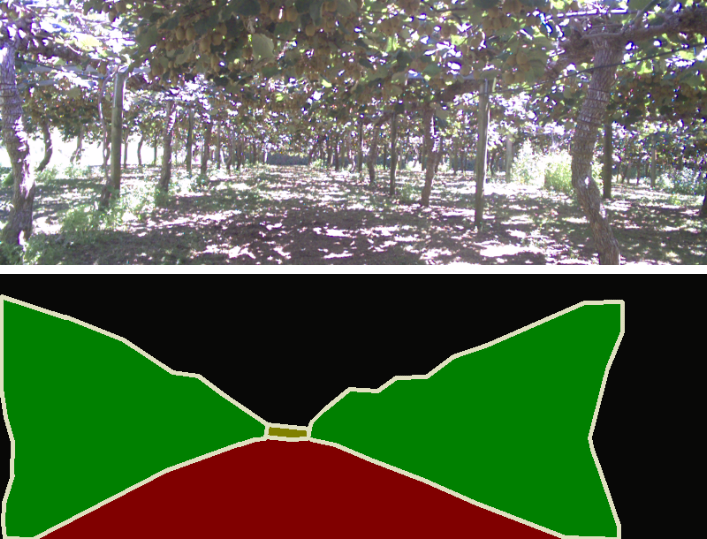
\includegraphics[width=\linewidth]{imgs/photos/segImgLabelPair_trimmed.png}
            % \includegraphics[width=\linewidth]{imgs/photos/segImg_sideBySide.png}
            \caption{
                An input image (top) and labeled output (bottom) used to train the semantic segmentation network.
            }
            \label{fig:segImgLabelPair}
        \end{figure}

        \begin{figure}[htb]
            \centering
            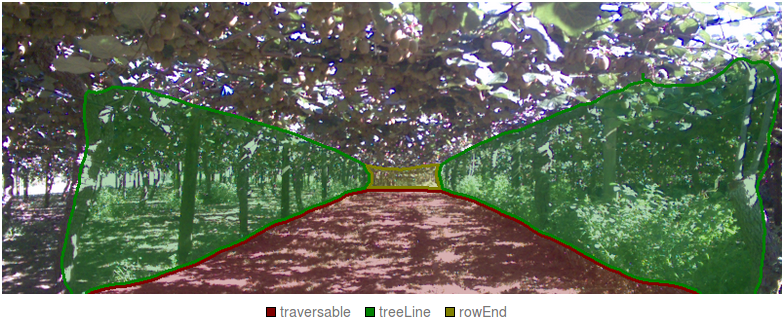
\includegraphics[width=\linewidth]{imgs/photos/semSegRowResults.png}
            \caption{
                An example inference result from the trained FCN-8s network.
            }
            \label{fig:semSegRowResults}
        \end{figure}

        Initially, individual trees and posts in the kiwifruit orchard were labeled.
    	It was later found that labeling the entire tree-line as a single class gave more robust results.
    	Objects labeled for this algorithm are:
        \begin{enumerate}
        \item traversable space (labeled as red),
        \item treelines (labeled as green), and
        \item the end of the current row (labeled as tan).
        \end{enumerate}
        Traversable space was defined as the ground area that the platform could drive directly to without collision.
        These labeled images were then used to train the FCN-8s network.
    	Sample output from the trained network is presented as figure \ref{fig:semSegRowResults}.

    % \subsubsection{Mapping and Localisation}
    %     An existing Simultaneous Localisation And Mapping (SLAM) package was used to test the multi-layer lidar.
    %     The package used was Gmapping \citep{Grisetti2007}, implemented as a ROS package \citep{Gerkey2010}.
    % 	Required input for Gmapping is odometry data and a single plane of lidar data.
    %     Odometry information was provided by the platform's in-built wheel encoders.

    %     \begin{figure}[htb]
    %         \centering
    %         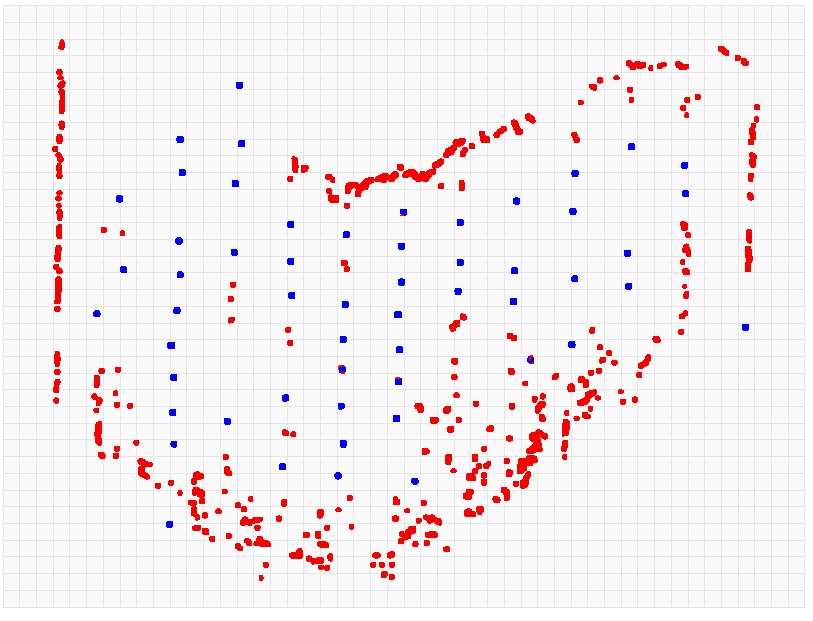
\includegraphics[width=\linewidth]{imgs/single_plane_extraction/single_plane_extraction.pdf}
    %         \caption{
    %             Processing of multi-layer lidar data into a single plane equivalent.
    %             Blue points are those selected by the algorithm for further processing, whereas red points are rejected.
    %         }
    %         \label{fig:singlePlaneExtraction}
    %     \end{figure}

    %     As the multi-layer lidar has 16 scanning layers, a conversion was necessary to produce the single plane of data required by Gmapping.
    %     The simplest conversion from multi-layer data to a single plane would be to select one of the available planes and discard the remaining data.
    %     However, that approach would loose any benefit offered by the multiple scanning layers.
    %     Instead, filtering the multi-layer data into a single plane was done by examining the centre four scan layers at each azimuth.
    %     With this algorithm, if the range difference between all four points at a single angle falls below a certain threshold, the closest point is returned.
    %     Alternatively, if the spread in points is above the threshold, no points are returned.
    %     This eliminates points from sloped or varying surfaces while still returning points from objects with vertical structure.
    %     The effect of this is that the orchard's structural elements remain visible, but ground and canopy information are removed.

    %     \begin{figure}[htb]
    %         \centering
    %         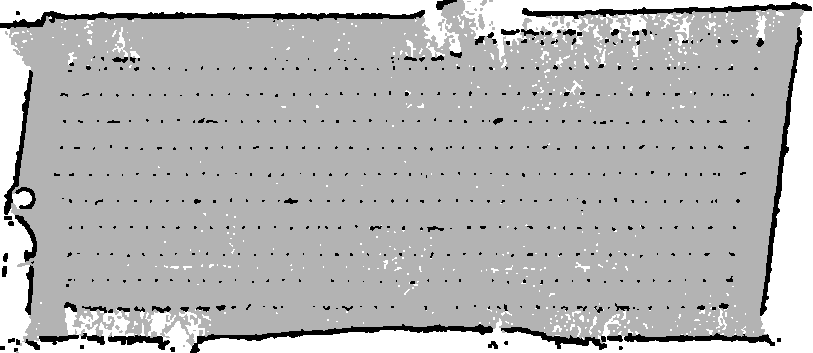
\includegraphics{imgs/gmapmap/gmapmap.pdf}
    %         \caption{
    %             A resulting SLAM based map of a kiwifruit orchard created using Gmapping.
    %             Data for the map was collected by traversing four of the orchard's ten rows.
    %             Odometry information has been taken from wheel encoders and a multi-layer lidar (Velodyle VLP-16).
    %         }
    %         \label{fig:gmapmap}
    %     \end{figure}

    %     The filtered points are then fed into Gmapping as a single plane with data from the platform's wheel encoders.
    %     Figure~\ref{fig:singlePlaneExtraction} shows the method's ability to filter structural elements from data containing significant canopy and ground reflections.
    %     Using this method, a SLAM based map of the orchard was created and is presented as figure \ref{fig:gmapmap}.


    % \subsubsection{Kiwifruit Orchard Row Tracking}
    %     \label{sect:row_tracking}

    %     Our final navigation test required interpreting the orchard's structure for the purpose of path generation.
    %     For this, a row guidance system was developed and tested.
    %     It uses the multi-layer to single-plane data filtering technique discussed previously.
    %     This algorithm also makes use of the platform's on-board wheel encoders.
    %     Details of this algorithm have been published separately \citep{Bell2016}.
    %     The key function of this algorithm is computing the angular offset of the platform from the row's centre-line.

    %     A visualisation of data captured whilst navigating the kiwifruit orchard is presented as figure \ref{fig:lastLidarFrame}.
    %     The method does not perform SLAM, so the visualised data represents only the sensor's current input, i.e., previous sensor data is not considered.
    %     Figure \ref{fig:lastLidarFrame} shows that while the algorithm is not perfect, it does perform reasonably well at identifying orchard structure and generating valid headings.

    %     \begin{figure}[htb]
    %         \centering
    %         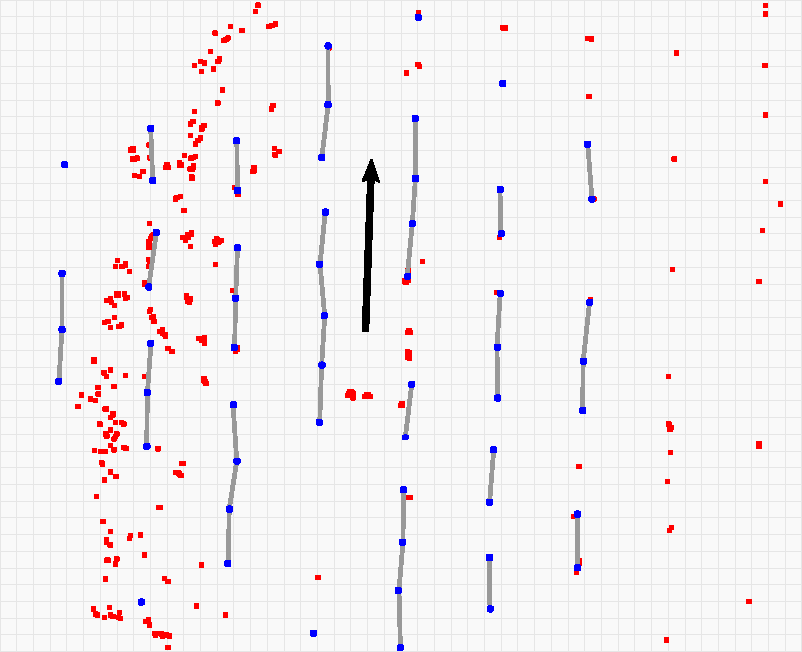
\includegraphics[width=\linewidth]{imgs/row_following/row_following_narrow.pdf}
    %         \caption{
    %             Row detection from multi-plane lidar data.
    %             Red points indicate non-structured data that have been ignored.
    %             Blue points indicate orchard structure data used for row navigation.
    %             Grey lines link orchard structure points by their nearest neighbors (performed algorithmically).
    %             The black arrow represents the centreline of the row current row.
    %         }
    %         \label{fig:lastLidarFrame}
    %     \end{figure}

\subsection{Sensor Selection Conclusions}
    The results from prototyped algorithms indicate that the multi-layer lidar and wheel encoder feedback are enough for mapping and localisation.
    This combination alone has proven successful for autonomous driving in kiwifruit orchards.
    A combination of 2D cameras and neural networking was suitable for object detection and classification.
    Further research toward using this as a means of generating a path for row following is underway and is expected to be published in future.

	% Object detection using a combination of colour cameras and neural networks in kiwifruit orchards .
	% Based on these results it was decided to continue testing cameras and multi-plane lidar as the primary sensors for the navigation system.
    % The autonomous driving algorithm described has been used to drive 20 km autonomously on three different robot platforms, including the AMMP, in two different kiwifruit orchards.
    % This driving was performed using just lidar and encoder data.


\section{Autonomous Driving}
\label{sect:autonomous}
    Using the row following algorithm developed for sensor testing, map based autonomous navigation of a kiwifruit orchard was implemented.
    Two key additions were required for the platform to navigate the orchard unassisted: the detection of a row's end and a method for turning between rows.

    The detection of a row's end is made by detecting a minimum volume of free space above the multi-layer lidar.
    Put simply, this equates to searching for a lack of canopy above the robot.
    This approach makes use of the multi-layer lidar, where layers above the horizontal are used as an `absence of canopy' detector.

    Turns between rows are performed by driving a series of set curvature movements while simultaneously performing lidar based obstacle avoidance.
    The series of set turns are recorded in a map file which are followed by the platform at the end of each row.
    A turn sequence sees the platform drive with a given steering angle for a given distance or until a given heading is achieved.
    Each row turn can contain any number of these sub-maneuvers.
    On completion of a turn, row following behavior is resumed which guides the platform through the row to the next turn.
    Figure \ref{fig:suzy_turning} shows the platform performing a row-end turn while under autonomous control.

    \begin{figure}[htb]
        \centering
        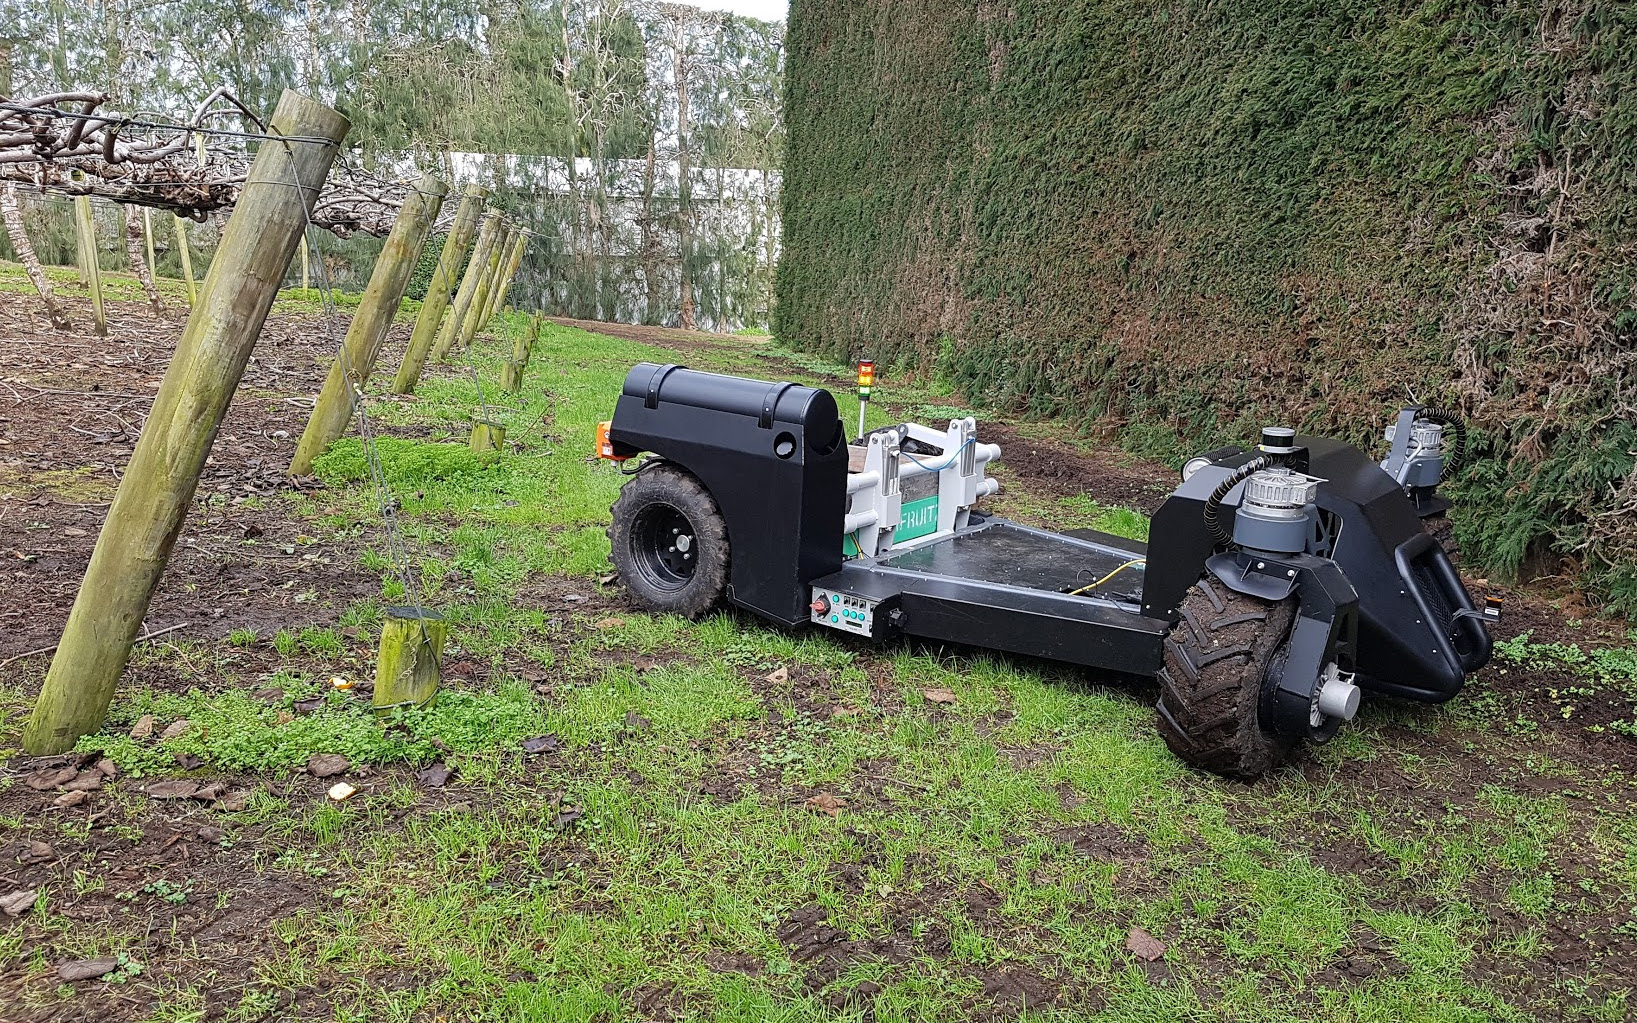
\includegraphics[width=\linewidth]{imgs/photos/suzy_turning.jpg}
        % 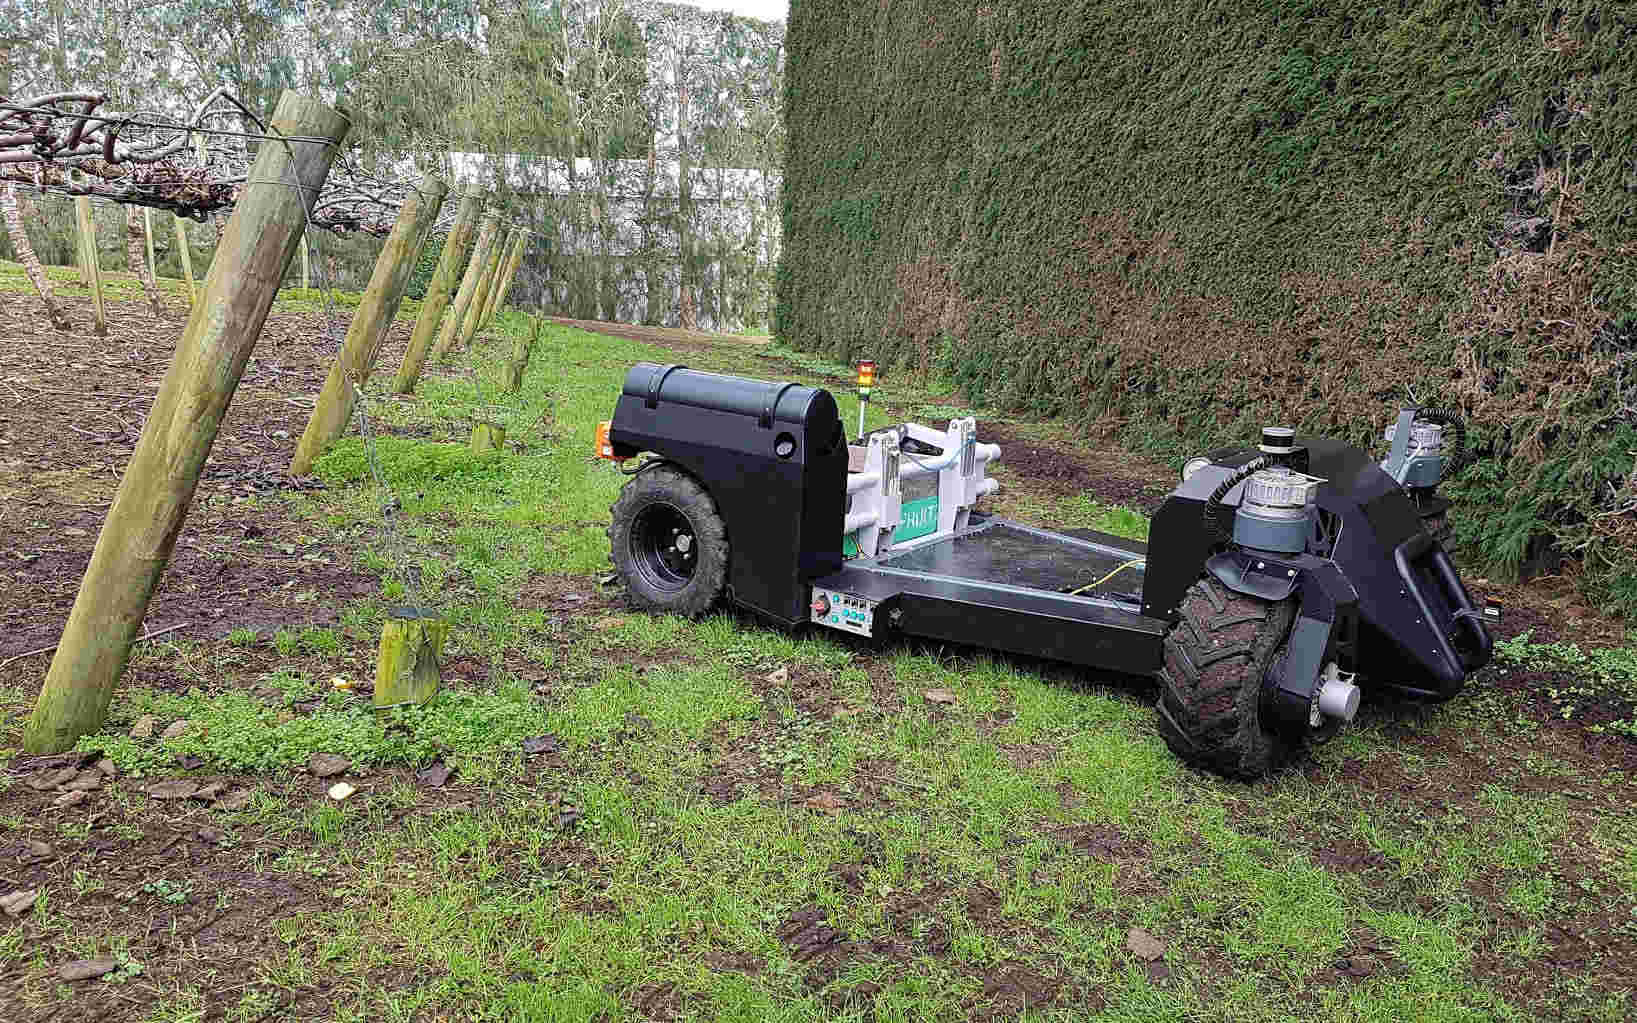
\includegraphics[width=\linewidth]{imgs/photos/suzy_turning_small.jpg}
        \caption{
            The platform performing a row-end turn in the headland area of a kiwifruit orchard while under autonomous control.
        }
        \label{fig:suzy_turning}
    \end{figure}

    Using the approaches developed here, the platform is routinely able to navigate two test orchards unassisted.
    Our primary test area is over \SI{1}{\kilo\meter} in total traversable length, spread over 10 rows.
    The developed algorithm has been used to autonomously control this platform and two smaller platforms through \SI{20}{\kilo\meter} of kiwifruit orchards.


\section{Conclusion}
    In this work, a platform designed specifically for driving through pergola style kiwifruit orchards has been presented.
    The platform has the capability of carrying a payload of up to \SI{1000}{\kilo\gram} through these orchards with minimal performance degradation.
    A \SI{48}{\volt} is identified as being a more sensible battery/bus voltage for development vehicles such as this, as opposed the \SI{96}{\volt} used here.
    This is due to safety reasons and increased availability of electrical hardware designed for this bus voltage.
    Sensors suitable for autonomous navigation have been selected, trialled and demonstrated as being useful as a means of navigating in this environment.
    Convolutional neural networks applied to monocular images proved to be a promising technique for row navigation and further work in this area is under-way.
    By processing multi-layer lidar data the platform presented here can reliably navigate an orchard block without human intervention.


\section*{Acknowledgements}
This research was supported by the New Zealand Ministry for Business, Innovation and Employment (MBIE) on contract UOAX1414.
The authors acknowledge contributions from Phillip Ross, Gordon Neshausen, Josh Barnett, and Erin Simms who were involved with the design and fabrication of the platform, and assistance testing and training neural networks from Nicky Penhall.


%% The Appendices part is started with the command \appendix;
%% appendix sections are then done as normal sections
%% \appendix

%% \section{}
%% \label{}

%% References
%%
%% Following citation commands can be used in the body text:
%%
%%  \citet{key}  ==>>  Jones et al. (1990)
%%  \citep{key}  ==>>  (Jones et al., 1990)
%%
%% Multiple citations as normal:
%% \citep{key1,key2}         ==>> (Jones et al., 1990; Smith, 1989)
%%                            or  (Jones et al., 1990, 1991)
%%                            or  (Jones et al., 1990a,b)
%% \cite{key} is the equivalent of \citet{key} in author-year mode
%%
%% Full author lists may be forced with \citet* or \citep*, e.g.
%%   \citep*{key}            ==>> (Jones, Baker, and Williams, 1990)
%%
%% Optional notes as:
%%   \citep[chap. 2]{key}    ==>> (Jones et al., 1990, chap. 2)
%%   \citep[e.g.,][]{key}    ==>> (e.g., Jones et al., 1990)
%%   \citep[see][pg. 34]{key}==>> (see Jones et al., 1990, pg. 34)
%%  (Note: in standard LaTeX, only one note is allowed, after the ref.
%%   Here, one note is like the standard, two make pre- and post-notes.)
%%
%%   \citealt{key}          ==>> Jones et al. 1990
%%   \citealt*{key}         ==>> Jones, Baker, and Williams 1990
%%   \citealp{key}          ==>> Jones et al., 1990
%%   \citealp*{key}         ==>> Jones, Baker, and Williams, 1990
%%
%% Additional citation possibilities
%%   \citeauthor{key}       ==>> Jones et al.
%%   \citeauthor*{key}      ==>> Jones, Baker, and Williams
%%   \citeyear{key}         ==>> 1990
%%   \citeyearpar{key}      ==>> (1990)
%%   \citetext{priv. comm.} ==>> (priv. comm.)
%%   \citenum{key}          ==>> 11 [non-superscripted]
%% Note: full author lists depends on whether the bib style supports them;
%%       if not, the abbreviated list is printed even when full requested.
%%
%% For names like della Robbia at the start of a sentence, use
%%   \Citet{dRob98}         ==>> Della Robbia (1998)
%%   \Citep{dRob98}         ==>> (Della Robbia, 1998)
%%   \Citeauthor{dRob98}    ==>> Della Robbia


%% References with bibTeX database:

\bibliographystyle{model5-names}
\bibliography{bibliography_jamie,bibliography_mark}


%% Authors are advised to submit their bibtex database files. They are
%% requested to list a bibtex style file in the manuscript if they do
%% not want to use model5-names.bst.

%% References without bibTeX database:

% \begin{thebibliography}{00}

%% \bibitem must have one of the following forms:
%%   \bibitem[Jones et al.(1990)]{key}...
%%   \bibitem[Jones et al.(1990)Jones, Baker, and Williams]{key}...
%%   \bibitem[Jones et al., 1990]{key}...
%%   \bibitem[\protect\citeauthoryear{Jones, Baker, and Williams}{Jones
%%       et al.}{1990}]{key}...
%%   \bibitem[\protect\citeauthoryear{Jones et al.}{1990}]{key}...
%%   \bibitem[\protect\astroncite{Jones et al.}{1990}]{key}...
%%   \bibitem[\protect\citename{Jones et al., }1990]{key}...
%%   \harvarditem[Jones et al.]{Jones, Baker, and Williams}{1990}{key}...
%%

% \bibitem[ ()]{}

% \end{thebibliography}

\end{document}

%%
%% End of file `elsarticle-template-5-harv.tex'.
